\chapter{Introduction}

% rapide résumé contexte, explication du sujet et pk avoir choisi le stage

%Intro contexte
\par
La peinture et le mouvement du regard de l'Homme ont toujours eu un lien étroit. En effet chaque spectateur regardera un tableau d'une manière différente de son voisin parce que chaque individu à sa propre culture, son propre point de vue, ... Pourtant la structure d'une peinture amènera le spectateur a suivre un sens de lecture. Celui-ci sera généralement commun à tous les spectateurs. Par exemple un individu qui découvre le tableau de La Joconde pour la première fois regardera presque systématiquement en premier lieu le visage de Mona Lisa et particulièrement ces yeux qui ont un effet particulier. Rare sont les personnes qui commenceront par identifier les éléments du décor en arrière-plan de la peinture.

\begin{figure}[h]
    \centering
    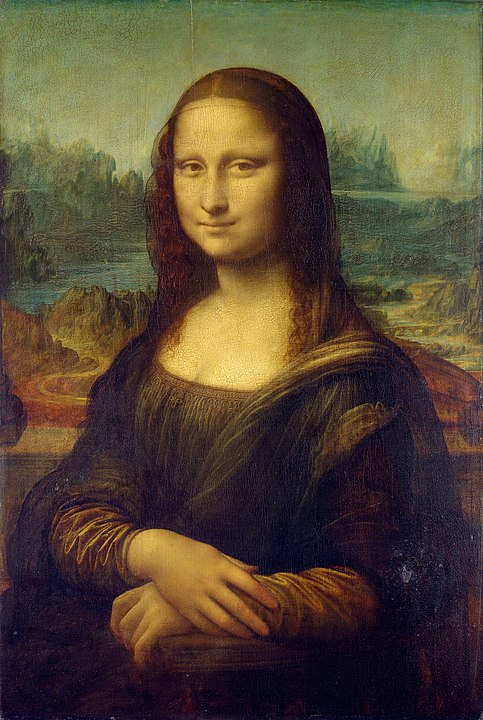
\includegraphics[width=0.3\textwidth]
                    {datas/Mona_Lisa_by_Leonardo_da_Vinci.jpg}
    \caption{La Joconde de Leonard de Vinci}
\end{figure}

%Intro saillance, Irisa et percept
\par
Ce sont l'ensemble de ces éléments qui attirent l'oeil humain qui constitue la saillance. C'est un élément important pour de nombreux domaines. On pense notamment au domaine du marketing et de la publicité qui doivent créer des affiches ou des spots publicitaires avec pour objectif d'attirer le plus possible le regard des consommateurs.

%Intro 
\par
La saillance dans la peinture permet d'analyser et de comprendre le regard humain ainsi que toutes les particularités qui en découlent. L'équipe Percept, équipe de recherche du laboratoire de l'IRISA, se penche sur le sujet et notamment à l'automatisation pour déterminer la saillance dans les peintures à l'aide de modèles de réseaux de neurones basés sur le machine learning.

%Explication du sujet de stage
\par
C'est là que le sujet de mon stage intervient. Cela consiste dans un premier temps à faire l'état de l'art des différents modèles qui existent sur des images naturelles. Dans un second temps le but est d'adapter le meilleur modèle pour qu'il s'adapte çà des peintures. Et enfin à partir des résultats de ce modèle trouver des applications visuelles et ludiques pour montrer l'intérêt d'un tel modèle.

%Explication comment j'ai trouvé le stage et quelles étaient mes motivations
\par 
Ce stage qui m'as été proposé par Olivier Le Meur correspondait à ce que je recherchais. C'est-à-dire un stage basé sur le machine learning, qui fait suite à mon projet industriel à l'ESIR qui consistait à générer des visages au moyen de réseau de neurones antagoniste génératif (GAN). Mais aussi un stage varié qui puisse me permettre de me former sur plusieurs compétences différentes.
% en conclusion : J'ai aimé la liberté et l'autonomie du stage, notamment les discussions qu'on a pu avoir avec Olivier pour déterminer quelles seraient les futur étapes du projet.




% \textit{Explication saillance, fixations, saccades, (top-down and bottum-up ?)}\\
% Bottom up : regard basé sur des signaux nerveux simple (contrast luminosité...)
% Top down : regard basé sur des éléments propre à l'individu et extérieur à l'image (connaissance, tache imposée...)
% ~\\
% Explication sujet :\\
% Base de données construite par stagiaires istic (a mettre dans contexte ?)\\
% saillance via machine learning\\
% Créer application pour mettre en valeur modèle saillance\\
% ~\\
% Pk avoir choisi le sujet\\